\documentclass[1p]{elsarticle_modified}
%\bibliographystyle{elsarticle-num}

%\usepackage[colorlinks]{hyperref}
%\usepackage{abbrmath_seonhwa} %\Abb, \Ascr, \Acal ,\Abf, \Afrak
\usepackage{amsfonts}
\usepackage{amssymb}
\usepackage{amsmath}
\usepackage{amsthm}
\usepackage{scalefnt}
\usepackage{amsbsy}
\usepackage{kotex}
\usepackage{caption}
\usepackage{subfig}
\usepackage{color}
\usepackage{graphicx}
\usepackage{xcolor} %% white, black, red, green, blue, cyan, magenta, yellow
\usepackage{float}
\usepackage{setspace}
\usepackage{hyperref}

\usepackage{tikz}
\usetikzlibrary{arrows}

\usepackage{multirow}
\usepackage{array} % fixed length table
\usepackage{hhline}

%%%%%%%%%%%%%%%%%%%%%
\makeatletter
\renewcommand*\env@matrix[1][\arraystretch]{%
	\edef\arraystretch{#1}%
	\hskip -\arraycolsep
	\let\@ifnextchar\new@ifnextchar
	\array{*\c@MaxMatrixCols c}}
\makeatother %https://tex.stackexchange.com/questions/14071/how-can-i-increase-the-line-spacing-in-a-matrix
%%%%%%%%%%%%%%%

\usepackage[normalem]{ulem}

\newcommand{\msout}[1]{\ifmmode\text{\sout{\ensuremath{#1}}}\else\sout{#1}\fi}
%SOURCE: \msout is \stkout macro in https://tex.stackexchange.com/questions/20609/strikeout-in-math-mode

\newcommand{\cancel}[1]{
	\ifmmode
	{\color{red}\msout{#1}}
	\else
	{\color{red}\sout{#1}}
	\fi
}

\newcommand{\add}[1]{
	{\color{blue}\uwave{#1}}
}

\newcommand{\replace}[2]{
	\ifmmode
	{\color{red}\msout{#1}}{\color{blue}\uwave{#2}}
	\else
	{\color{red}\sout{#1}}{\color{blue}\uwave{#2}}
	\fi
}

\newcommand{\Sol}{\mathcal{S}} %segment
\newcommand{\D}{D} %diagram
\newcommand{\A}{\mathcal{A}} %arc


%%%%%%%%%%%%%%%%%%%%%%%%%%%%%5 test

\def\sl{\operatorname{\textup{SL}}(2,\Cbb)}
\def\psl{\operatorname{\textup{PSL}}(2,\Cbb)}
\def\quan{\mkern 1mu \triangleright \mkern 1mu}

\theoremstyle{definition}
\newtheorem{thm}{Theorem}[section]
\newtheorem{prop}[thm]{Proposition}
\newtheorem{lem}[thm]{Lemma}
\newtheorem{ques}[thm]{Question}
\newtheorem{cor}[thm]{Corollary}
\newtheorem{defn}[thm]{Definition}
\newtheorem{exam}[thm]{Example}
\newtheorem{rmk}[thm]{Remark}
\newtheorem{alg}[thm]{Algorithm}

\newcommand{\I}{\sqrt{-1}}
\begin{document}

%\begin{frontmatter}
%
%\title{Boundary parabolic representations of knots up to 8 crossings}
%
%%% Group authors per affiliation:
%\author{Yunhi Cho} 
%\address{Department of Mathematics, University of Seoul, Seoul, Korea}
%\ead{yhcho@uos.ac.kr}
%
%
%\author{Seonhwa Kim} %\fnref{s_kim}}
%\address{Center for Geometry and Physics, Institute for Basic Science, Pohang, 37673, Korea}
%\ead{ryeona17@ibs.re.kr}
%
%\author{Hyuk Kim}
%\address{Department of Mathematical Sciences, Seoul National University, Seoul 08826, Korea}
%\ead{hyukkim@snu.ac.kr}
%
%\author{Seokbeom Yoon}
%\address{Department of Mathematical Sciences, Seoul National University, Seoul, 08826,  Korea}
%\ead{sbyoon15@snu.ac.kr}
%
%\begin{abstract}
%We find all boundary parabolic representation of knots up to 8 crossings.
%
%\end{abstract}
%\begin{keyword}
%    \MSC[2010] 57M25 
%\end{keyword}
%
%\end{frontmatter}

%\linenumbers
%\tableofcontents
%
\newcommand\colored[1]{\textcolor{white}{\rule[-0.35ex]{0.8em}{1.4ex}}\kern-0.8em\color{red} #1}%
%\newcommand\colored[1]{\textcolor{white}{ #1}\kern-2.17ex	\textcolor{white}{ #1}\kern-1.81ex	\textcolor{white}{ #1}\kern-2.15ex\color{red}#1	}

{\Large $\underline{12n_{0084}~(K12n_{0084})}$}

\setlength{\tabcolsep}{10pt}
\renewcommand{\arraystretch}{1.6}
\vspace{1cm}\begin{tabular}{m{100pt}>{\centering\arraybackslash}m{274pt}}
\multirow{5}{120pt}{
	\centering
	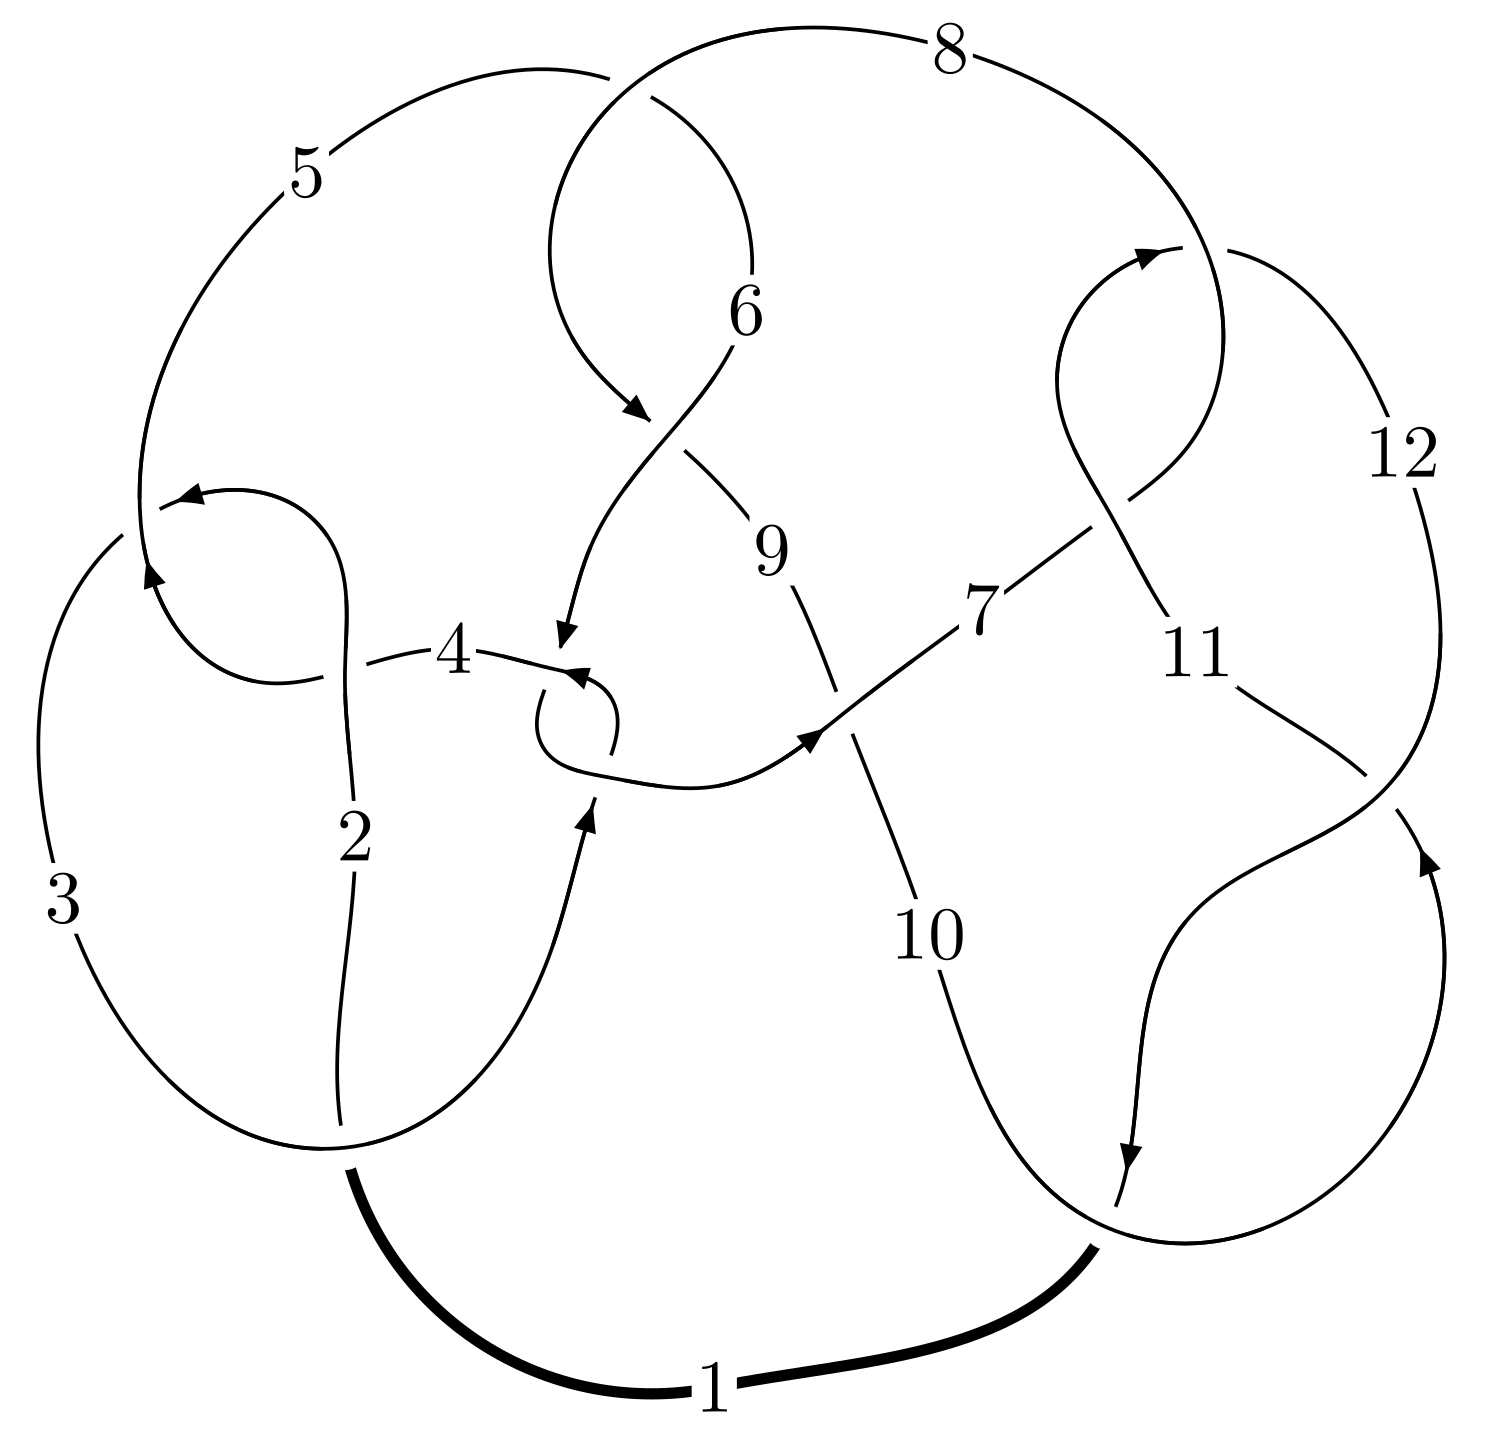
\includegraphics[width=112pt]{../../../GIT/diagram.site/Diagrams/png/2173_12n_0084.png}\\
\ \ \ A knot diagram\footnotemark}&
\allowdisplaybreaks
\textbf{Linearized knot diagam} \\
\cline{2-2}
 &
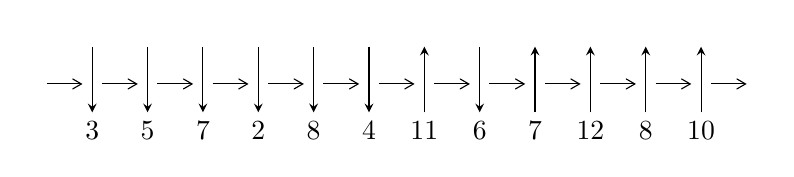
\begin{tikzpicture}[x=20pt, y=17pt]
	% nodes
	\node (C0) at (0, 0) {};
	\node (C1) at (1, 0) {};
	\node (C1U) at (1, +1) {};
	\node (C1D) at (1, -1) {3};

	\node (C2) at (2, 0) {};
	\node (C2U) at (2, +1) {};
	\node (C2D) at (2, -1) {5};

	\node (C3) at (3, 0) {};
	\node (C3U) at (3, +1) {};
	\node (C3D) at (3, -1) {7};

	\node (C4) at (4, 0) {};
	\node (C4U) at (4, +1) {};
	\node (C4D) at (4, -1) {2};

	\node (C5) at (5, 0) {};
	\node (C5U) at (5, +1) {};
	\node (C5D) at (5, -1) {8};

	\node (C6) at (6, 0) {};
	\node (C6U) at (6, +1) {};
	\node (C6D) at (6, -1) {4};

	\node (C7) at (7, 0) {};
	\node (C7U) at (7, +1) {};
	\node (C7D) at (7, -1) {11};

	\node (C8) at (8, 0) {};
	\node (C8U) at (8, +1) {};
	\node (C8D) at (8, -1) {6};

	\node (C9) at (9, 0) {};
	\node (C9U) at (9, +1) {};
	\node (C9D) at (9, -1) {7};

	\node (C10) at (10, 0) {};
	\node (C10U) at (10, +1) {};
	\node (C10D) at (10, -1) {12};

	\node (C11) at (11, 0) {};
	\node (C11U) at (11, +1) {};
	\node (C11D) at (11, -1) {8};

	\node (C12) at (12, 0) {};
	\node (C12U) at (12, +1) {};
	\node (C12D) at (12, -1) {10};
	\node (C13) at (13, 0) {};

	% arrows
	\draw[->,>={angle 60}]
	(C0) edge (C1) (C1) edge (C2) (C2) edge (C3) (C3) edge (C4) (C4) edge (C5) (C5) edge (C6) (C6) edge (C7) (C7) edge (C8) (C8) edge (C9) (C9) edge (C10) (C10) edge (C11) (C11) edge (C12) (C12) edge (C13) ;	\draw[->,>=stealth]
	(C1U) edge (C1D) (C2U) edge (C2D) (C3U) edge (C3D) (C4U) edge (C4D) (C5U) edge (C5D) (C6U) edge (C6D) (C7D) edge (C7U) (C8U) edge (C8D) (C9D) edge (C9U) (C10D) edge (C10U) (C11D) edge (C11U) (C12D) edge (C12U) ;
	\end{tikzpicture} \\
\hhline{~~} \\& 
\textbf{Solving Sequence} \\ \cline{2-2} 
 &
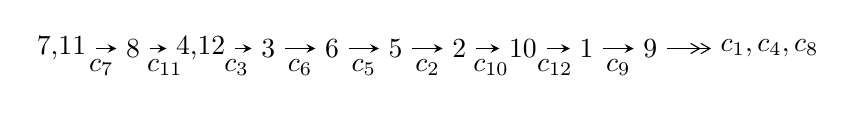
\begin{tikzpicture}[x=23pt, y=7pt]
	% node
	\node (A0) at (-1/8, 0) {7,11};
	\node (A1) at (1, 0) {8};
	\node (A2) at (33/16, 0) {4,12};
	\node (A3) at (25/8, 0) {3};
	\node (A4) at (33/8, 0) {6};
	\node (A5) at (41/8, 0) {5};
	\node (A6) at (49/8, 0) {2};
	\node (A7) at (57/8, 0) {10};
	\node (A8) at (65/8, 0) {1};
	\node (A9) at (73/8, 0) {9};
	\node (C1) at (1/2, -1) {$c_{7}$};
	\node (C2) at (3/2, -1) {$c_{11}$};
	\node (C3) at (21/8, -1) {$c_{3}$};
	\node (C4) at (29/8, -1) {$c_{6}$};
	\node (C5) at (37/8, -1) {$c_{5}$};
	\node (C6) at (45/8, -1) {$c_{2}$};
	\node (C7) at (53/8, -1) {$c_{10}$};
	\node (C8) at (61/8, -1) {$c_{12}$};
	\node (C9) at (69/8, -1) {$c_{9}$};
	\node (A10) at (11, 0) {$c_{1},c_{4},c_{8}$};

	% edge
	\draw[->,>=stealth]	
	(A0) edge (A1) (A1) edge (A2) (A2) edge (A3) (A3) edge (A4) (A4) edge (A5) (A5) edge (A6) (A6) edge (A7) (A7) edge (A8) (A8) edge (A9) ;
	\draw[->>,>={angle 60}]	
	(A9) edge (A10);
\end{tikzpicture} \\ 

\end{tabular} \\

\footnotetext{
The image of knot diagram is generated by the software ``\textbf{Draw programme}" developed by Andrew Bartholomew(\url{http://www.layer8.co.uk/maths/draw/index.htm\#Running-draw}), where we modified some parts for our purpose(\url{https://github.com/CATsTAILs/LinksPainter}).
}\phantom \\ \newline 
\centering \textbf{Ideals for irreducible components\footnotemark of $X_{\text{par}}$} 
 
\begin{align*}
I^u_{1}&=\langle 
-16510225313889 u^{40}-73379619742180 u^{39}+\cdots+7015565688188 b+16563398292357,\\
\phantom{I^u_{1}}&\phantom{= \langle  }-39282009802613 u^{40}-170243595424532 u^{39}+\cdots+7015565688188 a+73325296186875,\\
\phantom{I^u_{1}}&\phantom{= \langle  }u^{41}+5 u^{40}+\cdots+5 u-1\rangle \\
I^u_{2}&=\langle 
- u^2 a-2 u^2+b+a+u+2,\;a^2+2 a u+4 u^2+a-4 u+4,\;u^3- u^2+1\rangle \\
I^u_{3}&=\langle 
u^2+b,\;a- u,\;u^3- u^2+1\rangle \\
I^u_{4}&=\langle 
b,\;a+1,\;u+1\rangle \\
\\
\end{align*}
\raggedright * 4 irreducible components of $\dim_{\mathbb{C}}=0$, with total 51 representations.\\
\footnotetext{All coefficients of polynomials are rational numbers. But the coefficients are sometimes approximated in decimal forms when there is not enough margin.}
\newpage
\renewcommand{\arraystretch}{1}
\centering \section*{I. $I^u_{1}= \langle -1.65\times10^{13} u^{40}-7.34\times10^{13} u^{39}+\cdots+7.02\times10^{12} b+1.66\times10^{13},\;-3.93\times10^{13} u^{40}-1.70\times10^{14} u^{39}+\cdots+7.02\times10^{12} a+7.33\times10^{13},\;u^{41}+5 u^{40}+\cdots+5 u-1 \rangle$}
\flushleft \textbf{(i) Arc colorings}\\
\begin{tabular}{m{7pt} m{180pt} m{7pt} m{180pt} }
\flushright $a_{7}=$&$\begin{pmatrix}1\\0\end{pmatrix}$ \\
\flushright $a_{11}=$&$\begin{pmatrix}0\\u\end{pmatrix}$ \\
\flushright $a_{8}=$&$\begin{pmatrix}1\\- u^2\end{pmatrix}$ \\
\flushright $a_{4}=$&$\begin{pmatrix}5.59926 u^{40}+24.2666 u^{39}+\cdots+36.6437 u-10.4518\\2.35337 u^{40}+10.4595 u^{39}+\cdots+18.2641 u-2.36095\end{pmatrix}$ \\
\flushright $a_{12}=$&$\begin{pmatrix}u\\- u^3+u\end{pmatrix}$ \\
\flushright $a_{3}=$&$\begin{pmatrix}7.95264 u^{40}+34.7261 u^{39}+\cdots+54.9078 u-12.8128\\2.35337 u^{40}+10.4595 u^{39}+\cdots+18.2641 u-2.36095\end{pmatrix}$ \\
\flushright $a_{6}=$&$\begin{pmatrix}-0.679973 u^{40}-2.74952 u^{39}+\cdots-2.24406 u+4.15673\\0.448072 u^{40}+2.09737 u^{39}+\cdots-2.27213 u-0.275451\end{pmatrix}$ \\
\flushright $a_{5}=$&$\begin{pmatrix}-0.0387129 u^{40}-1.20772 u^{39}+\cdots-8.44788 u+4.53163\\-1.39663 u^{40}-6.29046 u^{39}+\cdots-11.2359 u+1.38905\end{pmatrix}$ \\
\flushright $a_{2}=$&$\begin{pmatrix}5.78006 u^{40}+24.1415 u^{39}+\cdots+36.8035 u-7.87601\\1.39663 u^{40}+6.29046 u^{39}+\cdots+11.2359 u-1.38905\end{pmatrix}$ \\
\flushright $a_{10}=$&$\begin{pmatrix}- u^3\\u^5- u^3+u\end{pmatrix}$ \\
\flushright $a_{1}=$&$\begin{pmatrix}u^5+u\\- u^7+u^5-2 u^3+u\end{pmatrix}$ \\
\flushright $a_{9}=$&$\begin{pmatrix}- u^5- u\\u^5- u^3+u\end{pmatrix}$\\&\end{tabular}
\flushleft \textbf{(ii) Obstruction class $= -1$}\\~\\
\flushleft \textbf{(iii) Cusp Shapes $= \frac{93247797228429}{1753891422047} u^{40}+\frac{1555830189736099}{7015565688188} u^{39}+\cdots+\frac{2808560039807687}{7015565688188} u-\frac{263248389242609}{3507782844094}$}\\~\\
\newpage\renewcommand{\arraystretch}{1}
\flushleft \textbf{(iv) u-Polynomials at the component}\newline \\
\begin{tabular}{m{50pt}|m{274pt}}
Crossings & \hspace{64pt}u-Polynomials at each crossing \\
\hline $$\begin{aligned}c_{1}\end{aligned}$$&$\begin{aligned}
&u^{41}+29 u^{40}+\cdots+71 u+1
\end{aligned}$\\
\hline $$\begin{aligned}c_{2},c_{4}\end{aligned}$$&$\begin{aligned}
&u^{41}-5 u^{40}+\cdots+7 u-1
\end{aligned}$\\
\hline $$\begin{aligned}c_{3},c_{6}\end{aligned}$$&$\begin{aligned}
&u^{41}-4 u^{40}+\cdots-10 u+2
\end{aligned}$\\
\hline $$\begin{aligned}c_{5},c_{8}\end{aligned}$$&$\begin{aligned}
&u^{41}-4 u^{40}+\cdots+512 u-512
\end{aligned}$\\
\hline $$\begin{aligned}c_{7},c_{11}\end{aligned}$$&$\begin{aligned}
&u^{41}-5 u^{40}+\cdots+5 u+1
\end{aligned}$\\
\hline $$\begin{aligned}c_{9}\end{aligned}$$&$\begin{aligned}
&u^{41}+3 u^{40}+\cdots-19597 u+2017
\end{aligned}$\\
\hline $$\begin{aligned}c_{10},c_{12}\end{aligned}$$&$\begin{aligned}
&u^{41}-9 u^{40}+\cdots+95 u-1
\end{aligned}$\\
\hline
\end{tabular}\\~\\
\newpage\renewcommand{\arraystretch}{1}
\flushleft \textbf{(v) Riley Polynomials at the component}\newline \\
\begin{tabular}{m{50pt}|m{274pt}}
Crossings & \hspace{64pt}Riley Polynomials at each crossing \\
\hline $$\begin{aligned}c_{1}\end{aligned}$$&$\begin{aligned}
&y^{41}-29 y^{40}+\cdots+1223 y-1
\end{aligned}$\\
\hline $$\begin{aligned}c_{2},c_{4}\end{aligned}$$&$\begin{aligned}
&y^{41}-29 y^{40}+\cdots+71 y-1
\end{aligned}$\\
\hline $$\begin{aligned}c_{3},c_{6}\end{aligned}$$&$\begin{aligned}
&y^{41}+42 y^{39}+\cdots+56 y-4
\end{aligned}$\\
\hline $$\begin{aligned}c_{5},c_{8}\end{aligned}$$&$\begin{aligned}
&y^{41}-50 y^{40}+\cdots+6160384 y-262144
\end{aligned}$\\
\hline $$\begin{aligned}c_{7},c_{11}\end{aligned}$$&$\begin{aligned}
&y^{41}-9 y^{40}+\cdots+95 y-1
\end{aligned}$\\
\hline $$\begin{aligned}c_{9}\end{aligned}$$&$\begin{aligned}
&y^{41}+135 y^{40}+\cdots+36517343 y-4068289
\end{aligned}$\\
\hline $$\begin{aligned}c_{10},c_{12}\end{aligned}$$&$\begin{aligned}
&y^{41}+51 y^{40}+\cdots+6127 y-1
\end{aligned}$\\
\hline
\end{tabular}\\~\\
\newpage\flushleft \textbf{(vi) Complex Volumes and Cusp Shapes}
$$\begin{array}{c|c|c}  
\text{Solutions to }I^u_{1}& \I (\text{vol} + \sqrt{-1}CS) & \text{Cusp shape}\\
 \hline 
\begin{aligned}
u &= \phantom{-}0.716889 + 0.703853 I \\
a &= -0.43425 - 2.19682 I \\
b &= -0.336317 + 0.798192 I\end{aligned}
 & -4.60661 + 1.52902 I & -5.50706 - 4.66307 I \\ \hline\begin{aligned}
u &= \phantom{-}0.716889 - 0.703853 I \\
a &= -0.43425 + 2.19682 I \\
b &= -0.336317 - 0.798192 I\end{aligned}
 & -4.60661 - 1.52902 I & -5.50706 + 4.66307 I \\ \hline\begin{aligned}
u &= -0.870049 + 0.467634 I \\
a &= -1.164530 + 0.454430 I \\
b &= \phantom{-}0.135790 - 0.918035 I\end{aligned}
 & \phantom{-}1.79473 + 0.06262 I & \phantom{-}2.65743 - 0.68980 I \\ \hline\begin{aligned}
u &= -0.870049 - 0.467634 I \\
a &= -1.164530 - 0.454430 I \\
b &= \phantom{-}0.135790 + 0.918035 I\end{aligned}
 & \phantom{-}1.79473 - 0.06262 I & \phantom{-}2.65743 + 0.68980 I \\ \hline\begin{aligned}
u &= \phantom{-}0.356456 + 0.980218 I \\
a &= \phantom{-}0.282408 + 0.117731 I \\
b &= -1.039320 - 0.421414 I\end{aligned}
 & -7.17972 - 2.87745 I & -9.28722 + 2.69256 I \\ \hline\begin{aligned}
u &= \phantom{-}0.356456 - 0.980218 I \\
a &= \phantom{-}0.282408 - 0.117731 I \\
b &= -1.039320 + 0.421414 I\end{aligned}
 & -7.17972 + 2.87745 I & -9.28722 - 2.69256 I \\ \hline\begin{aligned}
u &= -0.670401 + 0.652476 I \\
a &= \phantom{-}1.010200 - 0.553099 I \\
b &= \phantom{-}0.446012 + 1.120950 I\end{aligned}
 & \phantom{-}0.97725 - 4.44119 I & -1.27945 + 4.71656 I \\ \hline\begin{aligned}
u &= -0.670401 - 0.652476 I \\
a &= \phantom{-}1.010200 + 0.553099 I \\
b &= \phantom{-}0.446012 - 1.120950 I\end{aligned}
 & \phantom{-}0.97725 + 4.44119 I & -1.27945 - 4.71656 I \\ \hline\begin{aligned}
u &= \phantom{-}0.940640 + 0.501809 I \\
a &= -0.02791 + 1.96139 I \\
b &= \phantom{-}0.687266 - 0.758448 I\end{aligned}
 & -0.70118 + 4.43572 I & -0.34738 - 6.39371 I \\ \hline\begin{aligned}
u &= \phantom{-}0.940640 - 0.501809 I \\
a &= -0.02791 - 1.96139 I \\
b &= \phantom{-}0.687266 + 0.758448 I\end{aligned}
 & -0.70118 - 4.43572 I & -0.34738 + 6.39371 I\\
 \hline 
 \end{array}$$\newpage$$\begin{array}{c|c|c}  
\text{Solutions to }I^u_{1}& \I (\text{vol} + \sqrt{-1}CS) & \text{Cusp shape}\\
 \hline 
\begin{aligned}
u &= \phantom{-}0.877966 + 0.643589 I \\
a &= \phantom{-}0.016521 + 1.234530 I \\
b &= -0.609480 - 0.518945 I\end{aligned}
 & -4.07708 + 3.51500 I & -8.28852 - 2.95507 I \\ \hline\begin{aligned}
u &= \phantom{-}0.877966 - 0.643589 I \\
a &= \phantom{-}0.016521 - 1.234530 I \\
b &= -0.609480 + 0.518945 I\end{aligned}
 & -4.07708 - 3.51500 I & -8.28852 + 2.95507 I \\ \hline\begin{aligned}
u &= -0.854623 + 0.159200 I \\
a &= -0.978695 + 0.858024 I \\
b &= \phantom{-}0.041696 - 0.419660 I\end{aligned}
 & \phantom{-}1.46993 - 0.34552 I & \phantom{-}6.06026 + 0.56755 I \\ \hline\begin{aligned}
u &= -0.854623 - 0.159200 I \\
a &= -0.978695 - 0.858024 I \\
b &= \phantom{-}0.041696 + 0.419660 I\end{aligned}
 & \phantom{-}1.46993 + 0.34552 I & \phantom{-}6.06026 - 0.56755 I \\ \hline\begin{aligned}
u &= \phantom{-}0.877954 + 0.775956 I \\
a &= -0.968702 - 0.351197 I \\
b &= -0.598603 + 0.031599 I\end{aligned}
 & -3.83803 + 2.91878 I & \phantom{-}4.79738 - 5.00057 I \\ \hline\begin{aligned}
u &= \phantom{-}0.877954 - 0.775956 I \\
a &= -0.968702 + 0.351197 I \\
b &= -0.598603 - 0.031599 I\end{aligned}
 & -3.83803 - 2.91878 I & \phantom{-}4.79738 + 5.00057 I \\ \hline\begin{aligned}
u &= \phantom{-}0.537453 + 0.625371 I \\
a &= -0.426437 - 0.272772 I \\
b &= \phantom{-}0.891755 + 0.389086 I\end{aligned}
 & -2.04074 - 0.11127 I & -4.60725 + 0.35706 I \\ \hline\begin{aligned}
u &= \phantom{-}0.537453 - 0.625371 I \\
a &= -0.426437 + 0.272772 I \\
b &= \phantom{-}0.891755 - 0.389086 I\end{aligned}
 & -2.04074 + 0.11127 I & -4.60725 - 0.35706 I \\ \hline\begin{aligned}
u &= -0.802702\phantom{ +0.000000I} \\
a &= -5.09181\phantom{ +0.000000I} \\
b &= -0.275758\phantom{ +0.000000I}\end{aligned}
 & -0.345711\phantom{ +0.000000I} & -64.7260\phantom{ +0.000000I} \\ \hline\begin{aligned}
u &= \phantom{-}1.139710 + 0.532282 I \\
a &= \phantom{-}0.29262 - 1.64354 I \\
b &= -0.893901 + 0.701047 I\end{aligned}
 & -4.48025 + 8.31246 I & \phantom{-0.000000 } 0. - 7.85034 I\\
 \hline 
 \end{array}$$\newpage$$\begin{array}{c|c|c}  
\text{Solutions to }I^u_{1}& \I (\text{vol} + \sqrt{-1}CS) & \text{Cusp shape}\\
 \hline 
\begin{aligned}
u &= \phantom{-}1.139710 - 0.532282 I \\
a &= \phantom{-}0.29262 + 1.64354 I \\
b &= -0.893901 - 0.701047 I\end{aligned}
 & -4.48025 - 8.31246 I & \phantom{-0.000000 -}0. + 7.85034 I \\ \hline\begin{aligned}
u &= -1.26772\phantom{ +0.000000I} \\
a &= \phantom{-}0.964605\phantom{ +0.000000I} \\
b &= -0.640215\phantom{ +0.000000I}\end{aligned}
 & -0.787444\phantom{ +0.000000I} & -12.1570\phantom{ +0.000000I} \\ \hline\begin{aligned}
u &= -0.891473 + 0.933329 I \\
a &= -0.528554 + 0.154006 I \\
b &= \phantom{-}1.25025 - 1.10628 I\end{aligned}
 & -10.38260 + 1.04574 I & \phantom{-0.000000 } 0 \\ \hline\begin{aligned}
u &= -0.891473 - 0.933329 I \\
a &= -0.528554 - 0.154006 I \\
b &= \phantom{-}1.25025 + 1.10628 I\end{aligned}
 & -10.38260 - 1.04574 I & \phantom{-0.000000 } 0 \\ \hline\begin{aligned}
u &= -0.841724 + 0.990823 I \\
a &= \phantom{-}0.377207 - 0.291737 I \\
b &= -1.21490 + 1.06493 I\end{aligned}
 & -15.1663 + 7.0683 I & \phantom{-0.000000 } 0 \\ \hline\begin{aligned}
u &= -0.841724 - 0.990823 I \\
a &= \phantom{-}0.377207 + 0.291737 I \\
b &= -1.21490 - 1.06493 I\end{aligned}
 & -15.1663 - 7.0683 I & \phantom{-0.000000 } 0 \\ \hline\begin{aligned}
u &= -0.934438 + 0.935551 I \\
a &= -0.61279 + 1.51752 I \\
b &= -1.12955 - 1.22573 I\end{aligned}
 & -14.6673 - 1.5212 I & \phantom{-0.000000 } 0 \\ \hline\begin{aligned}
u &= -0.934438 - 0.935551 I \\
a &= -0.61279 - 1.51752 I \\
b &= -1.12955 + 1.22573 I\end{aligned}
 & -14.6673 + 1.5212 I & \phantom{-0.000000 } 0 \\ \hline\begin{aligned}
u &= -0.982434 + 0.885456 I \\
a &= \phantom{-}0.67122 - 1.65206 I \\
b &= \phantom{-}1.17691 + 1.18848 I\end{aligned}
 & -10.08510 - 7.74293 I & \phantom{-0.000000 } 0 \\ \hline\begin{aligned}
u &= -0.982434 - 0.885456 I \\
a &= \phantom{-}0.67122 + 1.65206 I \\
b &= \phantom{-}1.17691 - 1.18848 I\end{aligned}
 & -10.08510 + 7.74293 I & \phantom{-0.000000 } 0\\
 \hline 
 \end{array}$$\newpage$$\begin{array}{c|c|c}  
\text{Solutions to }I^u_{1}& \I (\text{vol} + \sqrt{-1}CS) & \text{Cusp shape}\\
 \hline 
\begin{aligned}
u &= -0.962450 + 0.919824 I \\
a &= \phantom{-}0.713562 - 0.200841 I \\
b &= -1.20978 + 1.14699 I\end{aligned}
 & -14.5747 - 5.2989 I & \phantom{-0.000000 } 0 \\ \hline\begin{aligned}
u &= -0.962450 - 0.919824 I \\
a &= \phantom{-}0.713562 + 0.200841 I \\
b &= -1.20978 - 1.14699 I\end{aligned}
 & -14.5747 + 5.2989 I & \phantom{-0.000000 } 0 \\ \hline\begin{aligned}
u &= \phantom{-}0.961309 + 0.961016 I \\
a &= -0.125970 + 0.554955 I \\
b &= \phantom{-}1.019520 - 0.111695 I\end{aligned}
 & -9.11622 + 3.51279 I & \phantom{-0.000000 } 0 \\ \hline\begin{aligned}
u &= \phantom{-}0.961309 - 0.961016 I \\
a &= -0.125970 - 0.554955 I \\
b &= \phantom{-}1.019520 + 0.111695 I\end{aligned}
 & -9.11622 - 3.51279 I & \phantom{-0.000000 } 0 \\ \hline\begin{aligned}
u &= -1.039620 + 0.876652 I \\
a &= -0.63077 + 1.75489 I \\
b &= -1.15233 - 1.13531 I\end{aligned}
 & -14.5120 - 13.9039 I & \phantom{-0.000000 } 0 \\ \hline\begin{aligned}
u &= -1.039620 - 0.876652 I \\
a &= -0.63077 - 1.75489 I \\
b &= -1.15233 + 1.13531 I\end{aligned}
 & -14.5120 + 13.9039 I & \phantom{-0.000000 } 0 \\ \hline\begin{aligned}
u &= \phantom{-}0.629652 + 0.060391 I \\
a &= -0.09621 + 3.42389 I \\
b &= \phantom{-}0.189078 - 1.367880 I\end{aligned}
 & \phantom{-}3.87413 + 2.95359 I & -12.9329 - 8.6631 I \\ \hline\begin{aligned}
u &= \phantom{-}0.629652 - 0.060391 I \\
a &= -0.09621 - 3.42389 I \\
b &= \phantom{-}0.189078 + 1.367880 I\end{aligned}
 & \phantom{-}3.87413 - 2.95359 I & -12.9329 + 8.6631 I \\ \hline\begin{aligned}
u &= -0.512134 + 0.182325 I \\
a &= \phantom{-}2.61667 + 0.05062 I \\
b &= \phantom{-}0.497781 - 0.337919 I\end{aligned}
 & -1.008150 - 0.694652 I & -6.89267 - 0.99274 I \\ \hline\begin{aligned}
u &= -0.512134 - 0.182325 I \\
a &= \phantom{-}2.61667 - 0.05062 I \\
b &= \phantom{-}0.497781 + 0.337919 I\end{aligned}
 & -1.008150 + 0.694652 I & -6.89267 + 0.99274 I\\
 \hline 
 \end{array}$$\newpage$$\begin{array}{c|c|c}  
\text{Solutions to }I^u_{1}& \I (\text{vol} + \sqrt{-1}CS) & \text{Cusp shape}\\
 \hline 
\begin{aligned}
u &= \phantom{-}0.113052\phantom{ +0.000000I} \\
a &= -3.84398\phantom{ +0.000000I} \\
b &= \phantom{-}0.612202\phantom{ +0.000000I}\end{aligned}
 & -1.00335\phantom{ +0.000000I} & -10.2280\phantom{ +0.000000I}\\
 \hline 
 \end{array}$$\newpage\newpage\renewcommand{\arraystretch}{1}
\centering \section*{II. $I^u_{2}= \langle - u^2 a-2 u^2+b+a+u+2,\;a^2+2 a u+4 u^2+a-4 u+4,\;u^3- u^2+1 \rangle$}
\flushleft \textbf{(i) Arc colorings}\\
\begin{tabular}{m{7pt} m{180pt} m{7pt} m{180pt} }
\flushright $a_{7}=$&$\begin{pmatrix}1\\0\end{pmatrix}$ \\
\flushright $a_{11}=$&$\begin{pmatrix}0\\u\end{pmatrix}$ \\
\flushright $a_{8}=$&$\begin{pmatrix}1\\- u^2\end{pmatrix}$ \\
\flushright $a_{4}=$&$\begin{pmatrix}a\\u^2 a+2 u^2- a- u-2\end{pmatrix}$ \\
\flushright $a_{12}=$&$\begin{pmatrix}u\\- u^2+u+1\end{pmatrix}$ \\
\flushright $a_{3}=$&$\begin{pmatrix}u^2 a+2 u^2- u-2\\u^2 a+2 u^2- a- u-2\end{pmatrix}$ \\
\flushright $a_{6}=$&$\begin{pmatrix}u^2 a- a u- a-3\\u^2 a+a u+3 u^2\end{pmatrix}$ \\
\flushright $a_{5}=$&$\begin{pmatrix}u^2 a- a u- a-3\\u^2 a+a u+3 u^2\end{pmatrix}$ \\
\flushright $a_{2}=$&$\begin{pmatrix}2 u^2 a+3 u^2- a-5\\u^2 a+a u+3 u^2\end{pmatrix}$ \\
\flushright $a_{10}=$&$\begin{pmatrix}- u^2+1\\- u^2\end{pmatrix}$ \\
\flushright $a_{1}=$&$\begin{pmatrix}-1\\0\end{pmatrix}$ \\
\flushright $a_{9}=$&$\begin{pmatrix}1\\- u^2\end{pmatrix}$\\&\end{tabular}
\flushleft \textbf{(ii) Obstruction class $= 1$}\\~\\
\flushleft \textbf{(iii) Cusp Shapes $= - u^2 a+15 a u+20 u^2+11 a+4 u+4$}\\~\\
\newpage\renewcommand{\arraystretch}{1}
\flushleft \textbf{(iv) u-Polynomials at the component}\newline \\
\begin{tabular}{m{50pt}|m{274pt}}
Crossings & \hspace{64pt}u-Polynomials at each crossing \\
\hline $$\begin{aligned}c_{1},c_{3},c_{9}\\c_{12}\end{aligned}$$&$\begin{aligned}
&(u^3- u^2+2 u-1)^2
\end{aligned}$\\
\hline $$\begin{aligned}c_{2},c_{11}\end{aligned}$$&$\begin{aligned}
&(u^3+u^2-1)^2
\end{aligned}$\\
\hline $$\begin{aligned}c_{4},c_{7}\end{aligned}$$&$\begin{aligned}
&(u^3- u^2+1)^2
\end{aligned}$\\
\hline $$\begin{aligned}c_{5},c_{8}\end{aligned}$$&$\begin{aligned}
&u^6
\end{aligned}$\\
\hline $$\begin{aligned}c_{6},c_{10}\end{aligned}$$&$\begin{aligned}
&(u^3+u^2+2 u+1)^2
\end{aligned}$\\
\hline
\end{tabular}\\~\\
\newpage\renewcommand{\arraystretch}{1}
\flushleft \textbf{(v) Riley Polynomials at the component}\newline \\
\begin{tabular}{m{50pt}|m{274pt}}
Crossings & \hspace{64pt}Riley Polynomials at each crossing \\
\hline $$\begin{aligned}c_{1},c_{3},c_{6}\\c_{9},c_{10},c_{12}\end{aligned}$$&$\begin{aligned}
&(y^3+3 y^2+2 y-1)^2
\end{aligned}$\\
\hline $$\begin{aligned}c_{2},c_{4},c_{7}\\c_{11}\end{aligned}$$&$\begin{aligned}
&(y^3- y^2+2 y-1)^2
\end{aligned}$\\
\hline $$\begin{aligned}c_{5},c_{8}\end{aligned}$$&$\begin{aligned}
&y^6
\end{aligned}$\\
\hline
\end{tabular}\\~\\
\newpage\flushleft \textbf{(vi) Complex Volumes and Cusp Shapes}
$$\begin{array}{c|c|c}  
\text{Solutions to }I^u_{2}& \I (\text{vol} + \sqrt{-1}CS) & \text{Cusp shape}\\
 \hline 
\begin{aligned}
u &= \phantom{-}0.877439 + 0.744862 I \\
a &= -1.06984 - 1.06527 I \\
b &= -0.215080 + 1.307140 I\end{aligned}
 & \phantom{-0.000000 -}5.65624 I & -3.29784 - 6.94206 I \\ \hline\begin{aligned}
u &= \phantom{-}0.877439 + 0.744862 I \\
a &= -1.68504 - 0.42445 I \\
b &= -0.569840\phantom{ +0.000000I}\end{aligned}
 & -4.13758 + 2.82812 I & -24.3518 + 2.3339 I \\ \hline\begin{aligned}
u &= \phantom{-}0.877439 - 0.744862 I \\
a &= -1.06984 + 1.06527 I \\
b &= -0.215080 - 1.307140 I\end{aligned}
 & \phantom{-0.000000 } -5.65624 I & -3.29784 + 6.94206 I \\ \hline\begin{aligned}
u &= \phantom{-}0.877439 - 0.744862 I \\
a &= -1.68504 + 0.42445 I \\
b &= -0.569840\phantom{ +0.000000I}\end{aligned}
 & -4.13758 - 2.82812 I & -24.3518 - 2.3339 I \\ \hline\begin{aligned}
u &= -0.754878\phantom{ +0.000000I} \\
a &= \phantom{-}0.25488 + 3.03873 I \\
b &= -0.215080 - 1.307140 I\end{aligned}
 & \phantom{-}4.13758 - 2.82812 I & \phantom{-}12.14969 - 2.71361 I \\ \hline\begin{aligned}
u &= -0.754878\phantom{ +0.000000I} \\
a &= \phantom{-}0.25488 - 3.03873 I \\
b &= -0.215080 + 1.307140 I\end{aligned}
 & \phantom{-}4.13758 + 2.82812 I & \phantom{-}12.14969 + 2.71361 I\\
 \hline 
 \end{array}$$\newpage\newpage\renewcommand{\arraystretch}{1}
\centering \section*{III. $I^u_{3}= \langle u^2+b,\;a- u,\;u^3- u^2+1 \rangle$}
\flushleft \textbf{(i) Arc colorings}\\
\begin{tabular}{m{7pt} m{180pt} m{7pt} m{180pt} }
\flushright $a_{7}=$&$\begin{pmatrix}1\\0\end{pmatrix}$ \\
\flushright $a_{11}=$&$\begin{pmatrix}0\\u\end{pmatrix}$ \\
\flushright $a_{8}=$&$\begin{pmatrix}1\\- u^2\end{pmatrix}$ \\
\flushright $a_{4}=$&$\begin{pmatrix}u\\- u^2\end{pmatrix}$ \\
\flushright $a_{12}=$&$\begin{pmatrix}u\\- u^2+u+1\end{pmatrix}$ \\
\flushright $a_{3}=$&$\begin{pmatrix}- u^2+u\\- u^2\end{pmatrix}$ \\
\flushright $a_{6}=$&$\begin{pmatrix}u^2\\- u^2+u+1\end{pmatrix}$ \\
\flushright $a_{5}=$&$\begin{pmatrix}u^2\\- u^2+u+1\end{pmatrix}$ \\
\flushright $a_{2}=$&$\begin{pmatrix}u-1\\- u^2+u+1\end{pmatrix}$ \\
\flushright $a_{10}=$&$\begin{pmatrix}- u^2+1\\- u^2\end{pmatrix}$ \\
\flushright $a_{1}=$&$\begin{pmatrix}-1\\0\end{pmatrix}$ \\
\flushright $a_{9}=$&$\begin{pmatrix}1\\- u^2\end{pmatrix}$\\&\end{tabular}
\flushleft \textbf{(ii) Obstruction class $= 1$}\\~\\
\flushleft \textbf{(iii) Cusp Shapes $= 2 u^2-3 u-2$}\\~\\
\newpage\renewcommand{\arraystretch}{1}
\flushleft \textbf{(iv) u-Polynomials at the component}\newline \\
\begin{tabular}{m{50pt}|m{274pt}}
Crossings & \hspace{64pt}u-Polynomials at each crossing \\
\hline $$\begin{aligned}c_{1},c_{3},c_{9}\\c_{12}\end{aligned}$$&$\begin{aligned}
&u^3- u^2+2 u-1
\end{aligned}$\\
\hline $$\begin{aligned}c_{2},c_{11}\end{aligned}$$&$\begin{aligned}
&u^3+u^2-1
\end{aligned}$\\
\hline $$\begin{aligned}c_{4},c_{7}\end{aligned}$$&$\begin{aligned}
&u^3- u^2+1
\end{aligned}$\\
\hline $$\begin{aligned}c_{5},c_{8}\end{aligned}$$&$\begin{aligned}
&u^3
\end{aligned}$\\
\hline $$\begin{aligned}c_{6},c_{10}\end{aligned}$$&$\begin{aligned}
&u^3+u^2+2 u+1
\end{aligned}$\\
\hline
\end{tabular}\\~\\
\newpage\renewcommand{\arraystretch}{1}
\flushleft \textbf{(v) Riley Polynomials at the component}\newline \\
\begin{tabular}{m{50pt}|m{274pt}}
Crossings & \hspace{64pt}Riley Polynomials at each crossing \\
\hline $$\begin{aligned}c_{1},c_{3},c_{6}\\c_{9},c_{10},c_{12}\end{aligned}$$&$\begin{aligned}
&y^3+3 y^2+2 y-1
\end{aligned}$\\
\hline $$\begin{aligned}c_{2},c_{4},c_{7}\\c_{11}\end{aligned}$$&$\begin{aligned}
&y^3- y^2+2 y-1
\end{aligned}$\\
\hline $$\begin{aligned}c_{5},c_{8}\end{aligned}$$&$\begin{aligned}
&y^3
\end{aligned}$\\
\hline
\end{tabular}\\~\\
\newpage\flushleft \textbf{(vi) Complex Volumes and Cusp Shapes}
$$\begin{array}{c|c|c}  
\text{Solutions to }I^u_{3}& \I (\text{vol} + \sqrt{-1}CS) & \text{Cusp shape}\\
 \hline 
\begin{aligned}
u &= \phantom{-}0.877439 + 0.744862 I \\
a &= \phantom{-}0.877439 + 0.744862 I \\
b &= -0.215080 - 1.307140 I\end{aligned}
 & \phantom{-0.000000 } 0 & -4.20216 + 0.37970 I \\ \hline\begin{aligned}
u &= \phantom{-}0.877439 - 0.744862 I \\
a &= \phantom{-}0.877439 - 0.744862 I \\
b &= -0.215080 + 1.307140 I\end{aligned}
 & \phantom{-0.000000 } 0 & -4.20216 - 0.37970 I \\ \hline\begin{aligned}
u &= -0.754878\phantom{ +0.000000I} \\
a &= -0.754878\phantom{ +0.000000I} \\
b &= -0.569840\phantom{ +0.000000I}\end{aligned}
 & \phantom{-0.000000 } 0 & \phantom{-}1.40430\phantom{ +0.000000I}\\
 \hline 
 \end{array}$$\newpage\newpage\renewcommand{\arraystretch}{1}
\centering \section*{IV. $I^u_{4}= \langle b,\;a+1,\;u+1 \rangle$}
\flushleft \textbf{(i) Arc colorings}\\
\begin{tabular}{m{7pt} m{180pt} m{7pt} m{180pt} }
\flushright $a_{7}=$&$\begin{pmatrix}1\\0\end{pmatrix}$ \\
\flushright $a_{11}=$&$\begin{pmatrix}0\\-1\end{pmatrix}$ \\
\flushright $a_{8}=$&$\begin{pmatrix}1\\-1\end{pmatrix}$ \\
\flushright $a_{4}=$&$\begin{pmatrix}-1\\0\end{pmatrix}$ \\
\flushright $a_{12}=$&$\begin{pmatrix}-1\\0\end{pmatrix}$ \\
\flushright $a_{3}=$&$\begin{pmatrix}-1\\0\end{pmatrix}$ \\
\flushright $a_{6}=$&$\begin{pmatrix}1\\0\end{pmatrix}$ \\
\flushright $a_{5}=$&$\begin{pmatrix}2\\-1\end{pmatrix}$ \\
\flushright $a_{2}=$&$\begin{pmatrix}-3\\1\end{pmatrix}$ \\
\flushright $a_{10}=$&$\begin{pmatrix}1\\-1\end{pmatrix}$ \\
\flushright $a_{1}=$&$\begin{pmatrix}-2\\1\end{pmatrix}$ \\
\flushright $a_{9}=$&$\begin{pmatrix}2\\-1\end{pmatrix}$\\&\end{tabular}
\flushleft \textbf{(ii) Obstruction class $= 1$}\\~\\
\flushleft \textbf{(iii) Cusp Shapes $= 0$}\\~\\
\newpage\renewcommand{\arraystretch}{1}
\flushleft \textbf{(iv) u-Polynomials at the component}\newline \\
\begin{tabular}{m{50pt}|m{274pt}}
Crossings & \hspace{64pt}u-Polynomials at each crossing \\
\hline $$\begin{aligned}c_{1},c_{2},c_{8}\\c_{9},c_{11},c_{12}\end{aligned}$$&$\begin{aligned}
&u-1
\end{aligned}$\\
\hline $$\begin{aligned}c_{3},c_{6}\end{aligned}$$&$\begin{aligned}
&u
\end{aligned}$\\
\hline $$\begin{aligned}c_{4},c_{5},c_{7}\\c_{10}\end{aligned}$$&$\begin{aligned}
&u+1
\end{aligned}$\\
\hline
\end{tabular}\\~\\
\newpage\renewcommand{\arraystretch}{1}
\flushleft \textbf{(v) Riley Polynomials at the component}\newline \\
\begin{tabular}{m{50pt}|m{274pt}}
Crossings & \hspace{64pt}Riley Polynomials at each crossing \\
\hline $$\begin{aligned}c_{1},c_{2},c_{4}\\c_{5},c_{7},c_{8}\\c_{9},c_{10},c_{11}\\c_{12}\end{aligned}$$&$\begin{aligned}
&y-1
\end{aligned}$\\
\hline $$\begin{aligned}c_{3},c_{6}\end{aligned}$$&$\begin{aligned}
&y
\end{aligned}$\\
\hline
\end{tabular}\\~\\
\newpage\flushleft \textbf{(vi) Complex Volumes and Cusp Shapes}
$$\begin{array}{c|c|c}  
\text{Solutions to }I^u_{4}& \I (\text{vol} + \sqrt{-1}CS) & \text{Cusp shape}\\
 \hline 
\begin{aligned}
u &= -1.00000\phantom{ +0.000000I} \\
a &= -1.00000\phantom{ +0.000000I} \\
b &= \phantom{-0.000000 } 0\end{aligned}
 & \phantom{-0.000000 } 0 & \phantom{-0.000000 } 0\\
 \hline 
 \end{array}$$\newpage
\newpage\renewcommand{\arraystretch}{1}
\centering \section*{ V. u-Polynomials}
\begin{tabular}{m{50pt}|m{274pt}}
Crossings & \hspace{64pt}u-Polynomials at each crossing \\
\hline $$\begin{aligned}c_{1}\end{aligned}$$&$\begin{aligned}
&(u-1)(u^3- u^2+2 u-1)^3(u^{41}+29 u^{40}+\cdots+71 u+1)
\end{aligned}$\\
\hline $$\begin{aligned}c_{2}\end{aligned}$$&$\begin{aligned}
&(u-1)(u^3+u^2-1)^3(u^{41}-5 u^{40}+\cdots+7 u-1)
\end{aligned}$\\
\hline $$\begin{aligned}c_{3}\end{aligned}$$&$\begin{aligned}
&u(u^3- u^2+2 u-1)^3(u^{41}-4 u^{40}+\cdots-10 u+2)
\end{aligned}$\\
\hline $$\begin{aligned}c_{4}\end{aligned}$$&$\begin{aligned}
&(u+1)(u^3- u^2+1)^3(u^{41}-5 u^{40}+\cdots+7 u-1)
\end{aligned}$\\
\hline $$\begin{aligned}c_{5}\end{aligned}$$&$\begin{aligned}
&u^9(u+1)(u^{41}-4 u^{40}+\cdots+512 u-512)
\end{aligned}$\\
\hline $$\begin{aligned}c_{6}\end{aligned}$$&$\begin{aligned}
&u(u^3+u^2+2 u+1)^3(u^{41}-4 u^{40}+\cdots-10 u+2)
\end{aligned}$\\
\hline $$\begin{aligned}c_{7}\end{aligned}$$&$\begin{aligned}
&(u+1)(u^3- u^2+1)^3(u^{41}-5 u^{40}+\cdots+5 u+1)
\end{aligned}$\\
\hline $$\begin{aligned}c_{8}\end{aligned}$$&$\begin{aligned}
&u^9(u-1)(u^{41}-4 u^{40}+\cdots+512 u-512)
\end{aligned}$\\
\hline $$\begin{aligned}c_{9}\end{aligned}$$&$\begin{aligned}
&(u-1)(u^3- u^2+2 u-1)^3(u^{41}+3 u^{40}+\cdots-19597 u+2017)
\end{aligned}$\\
\hline $$\begin{aligned}c_{10}\end{aligned}$$&$\begin{aligned}
&(u+1)(u^3+u^2+2 u+1)^3(u^{41}-9 u^{40}+\cdots+95 u-1)
\end{aligned}$\\
\hline $$\begin{aligned}c_{11}\end{aligned}$$&$\begin{aligned}
&(u-1)(u^3+u^2-1)^3(u^{41}-5 u^{40}+\cdots+5 u+1)
\end{aligned}$\\
\hline $$\begin{aligned}c_{12}\end{aligned}$$&$\begin{aligned}
&(u-1)(u^3- u^2+2 u-1)^3(u^{41}-9 u^{40}+\cdots+95 u-1)
\end{aligned}$\\
\hline
\end{tabular}\newpage\renewcommand{\arraystretch}{1}
\centering \section*{ VI. Riley Polynomials}
\begin{tabular}{m{50pt}|m{274pt}}
Crossings & \hspace{64pt}Riley Polynomials at each crossing \\
\hline $$\begin{aligned}c_{1}\end{aligned}$$&$\begin{aligned}
&(y-1)(y^3+3 y^2+2 y-1)^3(y^{41}-29 y^{40}+\cdots+1223 y-1)
\end{aligned}$\\
\hline $$\begin{aligned}c_{2},c_{4}\end{aligned}$$&$\begin{aligned}
&(y-1)(y^3- y^2+2 y-1)^3(y^{41}-29 y^{40}+\cdots+71 y-1)
\end{aligned}$\\
\hline $$\begin{aligned}c_{3},c_{6}\end{aligned}$$&$\begin{aligned}
&y(y^3+3 y^2+2 y-1)^3(y^{41}+42 y^{39}+\cdots+56 y-4)
\end{aligned}$\\
\hline $$\begin{aligned}c_{5},c_{8}\end{aligned}$$&$\begin{aligned}
&y^9(y-1)(y^{41}-50 y^{40}+\cdots+6160384 y-262144)
\end{aligned}$\\
\hline $$\begin{aligned}c_{7},c_{11}\end{aligned}$$&$\begin{aligned}
&(y-1)(y^3- y^2+2 y-1)^3(y^{41}-9 y^{40}+\cdots+95 y-1)
\end{aligned}$\\
\hline $$\begin{aligned}c_{9}\end{aligned}$$&$\begin{aligned}
&(y-1)(y^3+3 y^2+2 y-1)^3\\
&\cdot(y^{41}+135 y^{40}+\cdots+36517343 y-4068289)
\end{aligned}$\\
\hline $$\begin{aligned}c_{10},c_{12}\end{aligned}$$&$\begin{aligned}
&(y-1)(y^3+3 y^2+2 y-1)^3(y^{41}+51 y^{40}+\cdots+6127 y-1)
\end{aligned}$\\
\hline
\end{tabular}
\vskip 2pc
\end{document}